\chapter{战术导弹总体方案设计步骤以及数据流管理}
\section{战术导弹总体方案设计特点}
\begin{enumerate}[1.]
    \item 涉及学科专业多
    \item 涉及参数多
    \item 设计过程复杂
    \item 具有经验继承性
\end{enumerate}
\section{战术导弹总体方案设计}
\begin{enumerate}[1.]
\item 总体概要设计
    \begin{enumerate}[i]
        \item 确定弹身直径
        
        {\kaishu 最受关注的系统特征参数之一,导引头视场,导引头精度,发动机质量比,发动机工作效率,飞行阻力等都与之相关。}
        \item 确定战斗部类型
        \item 确定导弹速度方案
        
        {\kaishu 关键环节,根据目标运动,制导体制,导引方法,飞行时间约束设计,最终还有最小起飞质量约束。
        $9M311$导弹的例子(p21)很好的体现了设计师灵活性。
            三种基本形式:
                \begin{enumerate}[a]
                    \item 加速助推+无动力飞行
                    \item 加速助推+等速续航
                    \item 加速助推+加速续航+无动力飞行
                \end{enumerate}
        }
        \item 确定弹道方案
        \item 确定基本的动力系统形式
        
        {\kaishu 单室单推力$\rightarrow$速度方案一,剩余两个可由单室双推力或者两级串联,并联单室单推力发动机实现}
        \item 确定制导体制
        \item 确定导引规律
        \item 确定对发动机推进剂的性能要求
        \item 确定导弹的基本气动布局形式
        
        {\kaishu 鸭式布局,正常式,无尾式,旋转式}
        \item 确定导弹的基本控制模式
        
        {\kaishu STT转弯模式的基本控制模式:单,双以及三通道控制:
        
        三通道:俯仰,偏航,滚转稳定;
        
        双通道:无滚转控制,弹体低速旋转,两对控制舵面产生实时控制力
        
        单通道:弹体低速旋转,有一对控制执行机构,通过“弹体的低通滤波特性”形成周期平均控制力。
        }
    \end{enumerate}
\item 战斗部方案设计

\begin{figure}[h]
    \centering
    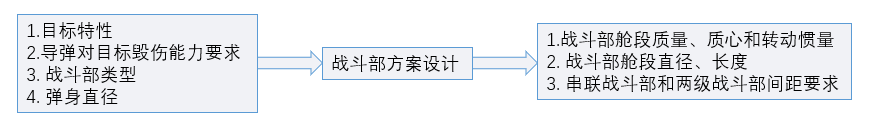
\includegraphics[scale = 0.75]{pictures/chapter3/1}
    \caption{战斗部方案设计输入输出}
    \label{wall_part}
\end{figure}
\item 起飞质量设计
    
\begin{figure}[h]
    \centering
    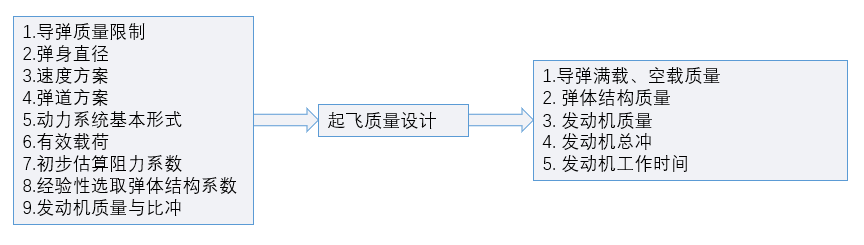
\includegraphics[scale = 0.75]{pictures/chapter3/2}
    \caption{起飞质量设计输入输出}
    \label{wall_part}
\end{figure}
\item 发动机方案设计

\begin{figure}[h]
    \centering
    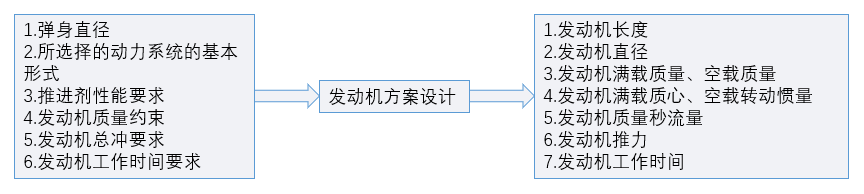
\includegraphics[scale = 0.75]{pictures/chapter3/3}
    \caption{发动机方案设计输入输出}
    \label{wall_part}
\end{figure}
\item 导引弹道运动学分析

\begin{figure}[h]
    \centering
    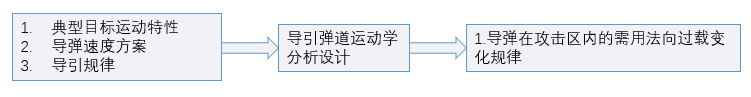
\includegraphics[scale = 0.75]{pictures/chapter3/4}
    \caption{导引弹道运动学分析输入输出}
    \label{wall_part}
\end{figure}
\item 控制系统概要设计

\begin{figure}[h]
    \centering
    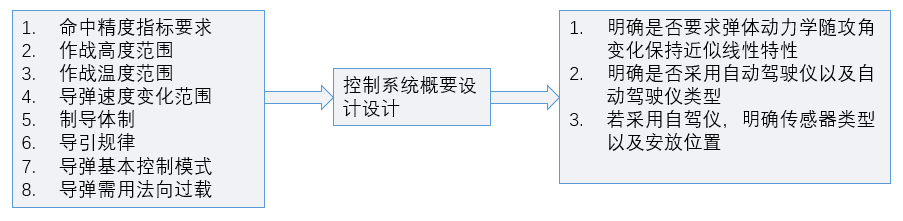
\includegraphics[scale = 0.75]{pictures/chapter3/5}
    \caption{发动机方案设计输入输出}
    \label{wall_part}
\end{figure}
\item 第一轮结构设计
\item 第一轮气动设计
\item 第二轮结构设计
\item 第二轮气动设计
\item 导引弹道动力学分析
\item 弹体动态特性分析
\item 制导回路设计
\item 自动驾驶仪设计
\item 有控刚体弹道仿真

\end{enumerate}

